% !TEX root = main.tex
\chapter{Introduction}

It's not rocket science.

Rocketry and its science is of great interest these last few years. Elon Musk and SpaceX's entry to the scene has propelled the science forward, with a goal of reaching the planet Mars within the coming years. The following paper contains an account of basic rocket design, with specific emphasis on discovering the the startup-sputtering of hybrid rocket engines, through thermal simulations. Thereto, calculations of thrust and simplification of the data collection technology is proceseed throughout the report.

My job has specifically been creating a multi-functional data collection device, by the use of a Raspberry Pi. Manometers and LAST-cells all connect to a single Raspberry Pi, which feeds the data to a computer. The Raspberry Pi is also used to set up the ignition system, which requires several layers of clearance before it can be ignited. The system starts data collection as soon as the rocket is armed, and accounts for all phases during the launch, eg. mentions when the rocket is started.

Data simulations are carried out in Engineering Equation Solver, henceforth known as EES. Gorm Andresen has provided previous experimental data, which has been used to calculate new boundary conditions. These new boundary conditions allows the calculation of sub-to supersonic flow, which may or may not reveal a sputtering effect.

\section{Basic Rocket Science}

A rocket consists of a few, very essential components. The basics of a rocket engine works by Newton's third law, where action and reaction push the rocket forward by expelling exhaust in the opposite direction.

\section{Nozzle Theory}

The nozzle consists of three parts: The combustion chamber, the converging into a throat, and diverging section after the throat. A rocket's effectivity is highly dependant on the shape, size and ratios between these three segments, and it is therefore essential to study these parts of the rocket design.
Hqwe
\begin{figure}
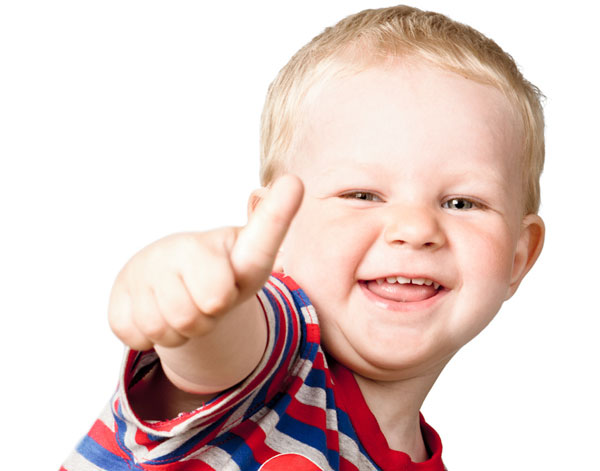
\includegraphics[width=\textwidth]{happy-boy}
\caption{det er nok at skrive filnavnet, for main.tex kigger efter figurer i /figures/}
\label{fig:yyy}
\end{figure}
